\documentclass[12pt]{article}

\author{David Gleich}
\title{Matlab BGL v2.1}
\date{5 April 2007}

\usepackage{color}
\definecolor{shadecolor}{rgb}{0.9,0.9,0.9} 
\usepackage{framed}
\usepackage{url}
\usepackage{graphicx}
\usepackage{amsmath}
\usepackage{tabularx}

\usepackage[bf]{caption}

\usepackage{listings}
\lstset{basicstyle={\footnotesize \ttfamily}, columns=flexible,
backgroundcolor=\color{shadecolor},frame=single,
rulesepcolor=\color{black},
xleftmargin=36pt}


%\renewcommand{\familydefault}{\sfdefault}
\usepackage{cmbright}
\usepackage{fullpage}
%\setlength{\textheight}{9in}
%\setlength{\topmargin}{-0.5in}
%\setlength{\textwidth}{6.5in}
%\setlength{\oddsidemargin}{0.125in}
%\setlength{\evensidemargin}{0.125in}

\setlength{\parindent}{0in}
\setlength{\parskip}{6pt}

\def\floatpagefraction{.9}      % default .5
\def\topfraction{.9}            % default .7
\def\bottomfraction{.9}         % default .3
\def\textfraction{.1}           % default .2

%\newcommand{\mcode}[1]{\parashade[.95]{roundcorners}{\begin{Verbatim}#1\end{Verbatim}}}
%\newenvironment{mcode}{\begin{lstlisting}}{\end{lstlisting}}
\lstnewenvironment{mcode}{}{}
\lstnewenvironment{mcode-small}{\lstset{basicstyle={\scriptsize \ttfamily}}}{}

\newcommand{\mycmd}[1]{\url{#1}}
\newcommand{\mypath}[1]{{\ttfamily \small #1}}
\DeclareRobustCommand\cs[1]{\texttt{\char`\\#1}} 
\newcommand{\mynote}[1]{\begin{center} \fbox{\hspace{1cm}\bfseries Note: #1\hspace{1cm}}\end{center}}

%\renewcommand{\maketitle}{

\begin{document}

%%% HTML-begin title
{
\setlength{\parskip}{0pt}
\begin{center}
{\Large Matlab BGL v2.1}\\
David Gleich\\
\today
\end{center}
%%% HTML-toc
}
%%% HTML-end title
\section*{Abstract and Synopsis}

MatlabBGL adds a wide range for graph algorithms to Matlab.  The graph algorithms come from the Boost Graph Library\footnote{\url{http://www.boost.org/doc/graph}}.  The following code segment briefly demonstrates some of the calls and algorithms in MatlabBGL.

\bigskip

\begin{mcode}
>> [d ft dt pred] = dfs(A)
>> [d dt pred] = bfs(A);

>> [d pred] = dijkstra_sp(A,u);
>> [d pred] = bellman_ford_sp(A,u);
>> [d pred] = dag_sp(A,u);
>> D = johnson_all_sp(A);
>> D = floyd_warshall_all_sp(A);

>> T = kruskal_mst(A);
>> T = prim_mst(A);

>> cc = components(A)  
>> [a C] = biconnected_components(A);

>> [flow cut R F] = max_flow(A,u,v);

>> print_func = @(str) @(u) fprintf('called %s(%s)\n', str, char(labels(u)));
>> breadth_first_search(A,1,struct('examine_vertex',print_func('examine_vertex')));

>> [d pred rank] = astar_search(A,u,heuristic_func);
\end{mcode}

\newpage
{
\setlength{\parskip}{0pt}
\tableofcontents
}
\newpage

\section{Installation}
We are distributing the library as a set of precompiled mex files for Windows and Linux along with the source code for the libraries.  This combination will work for all people, although it may take a bit of effort.

If all goes well, installing the library is as easy as:
\begin{enumerate}
\item	Unzip the file \url{matlab_bgl.zip}.  For the sake of example, let's assume you unzipped it into the same folder as I do: ``\mypath{/home/dgleich/matlab/}'' on Linux and ``\mypath{C:\cs{}Documents and Settings\cs{}dgleich\cs{}My Documents\cs{}matlab\cs{}}'' on Windows.
\item	In Matlab, add either the Linux path ``\mypath{/home/dgleich/matlab/matlab\_bgl/}'' or the Windows path ``\mypath{C:\cs{}Documents and Settings\cs{}dgleich\cs{}My Documents\cs{}matlab\cs{}}'' to the path (but replacing those directories with the ones where you actually unzipped \url{matlab_bgl.zip}).
\end{enumerate}

To test the installation, try running the following script.
\begin{mcode}
% add matlab_bgl to the path
% e.g. addpath('/home/dgleich/matlab/matlab_bgl');
>> clustering_coefficients(sparse(ones(5)))
ans =
     1
     1
     1
     1
     1
\end{mcode}
\subsection*{Building the library}
\mynote{You should not need to complete the following steps!}
In general, the precompiled versions should work.  If they do not and you would like to try compiling the mex files from source, this section explains the process.  On Windows, you must use a Microsoft Visual Studio compiler.  The free Visual Studio 2003 Compiler Toolkit\footnote{\url{http://msdn.microsoft.com/visualc/vctoolkit2003/}} suffices for this purpose.  On Linux, any recent version of gcc should work.  All the precompiled files are compiled with gcc-3.4 under Linux and the Microsoft Visual Studio 2003 compiler on 32-bit Windows and Microsoft Visual Studio 2005 x64 cross compiler for 64-bit Windows.

To compile the .lib or .a files, first determine which compile script you should use.  
\begin{center}
\begin{tabular}{lll}
\hline \hline
\textbf{System} & \textbf{Matlab} & \textbf{Script}\\
\hline
32-bit Windows & All & \mycmd{compile-win32.bat}\\
64-bit Windows & Matlab 7.3 - Current & \mycmd{compile-win64.bat}\\
32-bit Linux & Matlab 7.0 - Current & \mycmd{compile-linux-32.sh}\\
64-bit Linux & Matlab 7.0 - Matlab 7.2 & \mycmd{compile-linux-64.sh}\\
64-bit Linux & Matlab 7.3 - Current & \mycmd{compile-linux-64-large.sh}\\
Mac OS X (PPC) & Matlab 7.0 - Current & \mycmd{compile-macosx-ppc-32.sh}\\
Mac OS X (Intel) & Matlab 7.4 - Current & \mycmd{compile-macosx-intel-32.sh}\\
\hline
\end{tabular}
\end{center}
Next, you need to download and unzip version 1.33.1 of the Boost Graph Library.  Go to \url{http://www.boost.org} to download this code.  Update the script file for your platform with the correct path so that the \mycmd{BOOSTDIR} or \mycmd{BOOST_DIR} variable gives the correct location.  Check all the paths to the various tools on Windows to make sure they correspond to your installation.  
Finally, run the script file from the libmbgl directory.  For example, on 32-bit Windows
\begin{mcode}
E:\dev\matlab\download\matlab_bgl-2.1\libmbgl>compile-win32.bat
Setting environment for using Microsoft Visual Studio 2005 x86 tools.
Setting environment for using Microsoft Visual C++ 2003 Toolkit.
(If you have another version of Visual Studio or Visual C++ installed and wish
to use its tools from the command line, run vcvars32.bat for that version.)

Thank you for choosing the Visual C++ Toolkit 2003!  Get started quickly by
building the code samples included in the "Samples" directory.  Each sample
includes a short whitepaper discussing the Visual C++ features, and a batch
file for building the code.

Type "cl /?" for brief documentation on compiler options.

Visit http://msdn.microsoft.com/visualc/using/documentation/default.aspx for
complete compiler documentation.

E:\dev\matlab\download\MATLAB~1.1\libmbgl>cl -c -nologo -I"." -I"e:\dev\lib\boos
t_1_33_1" /Fo"Release\\" /EHsc /D "NDEBUG" /O2 /ML components.cc
components.cc

E:\dev\matlab\download\MATLAB~1.1\libmbgl>cl -c -nologo -I"." -I"e:\dev\lib\boos
t_1_33_1" /Fo"Release\\" /EHsc /D "NDEBUG" /O2 /ML max_flow.cc
max_flow.cc

...
\end{mcode}
On 64-bit Linux, 
\begin{mcode}
dgleich@icme-112-dgleich:matlab_bgl/libmbgl$ chmod u+x compile-linux-64-large.sh
dgleich@icme-112-dgleich:matlab_bgl/libmbgl$ ./compile-linux-64-large.sh
...
\end{mcode}

To compile the mex files from the .lib or .a files, 
\begin{mcode}
>> cd /home/dgleich/matlab/ % use your directory here instead of mine!
>> cd matlab_bgl/
>> cd private
>> compile
>> cd ..
>> cd @ipdouble
>> mex subsasgn.c
>> cd ..
>> cd @ipint32
>> mex subsasgn.c
>> cd ..
\end{mcode}
If you cannot compile the library and the example does not work, please send email to \url{mithandor@gmail.com} with as much output as you can.  

Here are a few hints if you have problems.
\begin{itemize}
\item Try running \mycmd{mex~-setup} and selecting the \mycmd{gcc} or Microsoft Visual Studio compiler setup for Linux and Windows, respectively.
\item For Linux, edit your mexopts.sh file and remove the \mycmd{-ansi} flag from the CFLAGS and CXXFLAGS for your platform.
\item For some versions of Matlab, you may want to change the \mycmd{CC} and \mycmd{CXX} to gcc-3.4 or gcc-4.0.
\end{itemize}

\section{Motivation and Implementation}
The Boost Graph Library\footnote{\url{http://www.boost.org/libs/graph/doc/}} is a powerful graph analysis toolkit.  It contains efficient algorithms implemented as generic C++ template specifications.  In the MatlabBGL library, we have wrapped these algorithms with \emph{mex} functions which are callable from Matlab.  The goal of the library was to introduce as little new material in Matlab as possible.  As the next section explains, MatlabBGL uses the Matlab sparse matrix type as the graph type directly.

The idea behind the MatlabBGL library is to provide a rich set of graph-theoretic routines as efficient Matlab functions.  

\subsection{Graphs in Matlab}
Matlab \emph{has} a built in graph type: the sparse matrix.  The goal of the MatlabBGL library is to use the Matlab sparse matrix as a graph type.  To be slightly more concrete, we use a sparse matrix in Matlab to represent the adjacency matrix of two graphs from the Boost Graph library review of graph theory.

\begin{figure}[ht!]
\centering
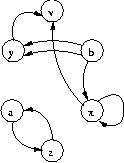
\includegraphics[width=1.5in]{digraph}
\caption{A directed graph.}
\label{fig:digraph}
\end{figure}

For the graph in Figure~\ref{fig:digraph}, the adjacency matrix is 
\[ \begin{pmatrix}
     0  &    0  &   0  &   0  &   0 &    1\\
     0  &   0  &   0   &  1  &   2  &   0\\
     0  &   0  &   0   &  0  &   0  &   0\\
     0  &   0  &   0   &  1  &   0  &   1\\
     0  &   0  &   1   &  0  &   0  &   0\\
     1  &   0  &   0   &  0  &   0  &   0\\
     \end{pmatrix},\]
and we labeled vertex $a=1$, $b=2$, $v=3$, $x=4$, $y=5$, $z=6$.  In the original graph from Figure~\ref{fig:digraph}, there are two edges from $b$ to $y$.  We have replaced both edges with a two in the adjacency matrix.  While this works for many algorithms, there are currently no ways of implemented true multi-graphs in MatlabBGL.

\mynote{There are currently no multi-graphs supported in MatlabBGL.}

We can construct this graph as a Matlab sparse matrix with the following set of commands.

\begin{mcode}
>> A = sparse(6,6);
>> A(1,6) = 1;
>> A(6,1) = 1;
>> A(2,4) = 1;
>> A(2,5) = 2;
>> A(4,4) = 1;
>> A(4,6) = 1;
>> A(5,3) = 1;
>> labels = {'a';'b';'v';'x';'y';'z'};
\end{mcode}

Now, we can use the directed graph as a Matlab sparse matrix and as a MatlabBGL graph.  As we will see, we can treat any square sparse matrix as a MatlabBGL graphs.

\begin{figure}[ht!]
\centering
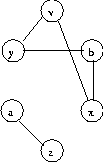
\includegraphics[width=1.5in]{undigraph}
\caption{An undirected graph.}
\label{fig:undigraph}
\end{figure}

MatlabBGL requires that undirected graphs have symmetric adjacency.  When constructing a graph, this means that you must specify each edge twice.  The following Matlab session constructs the graph in Figure~\ref{fig:undigraph}.

\begin{mcode}
>> A = sparse(6,6);
>> A(1,6) = 1;
>> A(6,1) = 1;
>> A(2,4) = 1;
>> A(4,2) = 1;
>> A(2,5) = 1;
>> A(5,2) = 1;
>> A(3,4) = 1;
>> A(4,3) = 1;
>> A(3,5) = 1;
>> A(5,3) = 1;
>> labels = {'a';'b';'v';'x';'y';'z'};
\end{mcode}

An easier way of constructed the graph from Figure~\ref{fig:undigraph} is to take advantage of some of Matlab's sparse matrix routines.  We can use one command to add a reverse edge for each edge listed in a sparse matrix by executing
\begin{mcode}
>> A = max(A,A');
\end{mcode}

Using this command, we can build the undirected graph using the commands:
\begin{mcode}
>> A = sparse(6,6);
>> A(1,6) = 1;
>> A(2,4) = 1;
>> A(5,2) = 1;
>> A(4,3) = 1;
>> A(3,5) = 1;
>> A = max(A,A');
\end{mcode}

In general, any square sparse matrix in Matlab is a MatlabBGL graph; the non-zeros of the matrix define the edges.  If the sparse matrix is symmetric, then the graph is undirected.

\mynote{Any square sparse matrix is a MatlabBGL graph.}




\subsection{Implementation details}
\label{ref:impl-details}
In this section, we will address some fairly technical details of the implementation.  Matlab implements sparse matrices as a set of compressed column arrays.  Most adjacency matrix representations (and the one used in MatlabBGL) use the rows of the matrix to specify the edges from a particular vertex.  That is, $A(i,j) = 1$ indices there is an edge between vertex $i$ and vertex $j$.  

Unfortunately, this means that in the Matlab compressed column storage format, we do not have efficient access to the elements of each row of the matrix (i.e. the adjacent vertices).  The Boost graph algorithms require access to the adjacent vertices.  So, every time we call a MatlabBGL function we transpose the sparse matrix, unless the function requires a symmetric input.

Some algorithms only use the non-zero structure of the sparse matrix.  Other algorithms use the values of the non-zeros as the weights of the edges.  In general, things work the way you expect them to using a sparse adjacency matrix to represent the graph; we have documented any serious deviations from the expected behavior.

Transposing the matrix can be somewhat expensive, so we provide an option to eliminate the transpose \emph{if the user knows better}.  Thus, for the most efficient MatlabBGL runtimes, construct the transpose of the adjacency matrix and run the MatlabBGL routines with the extra option 
\begin{mcode}
>> bfs(A,u,struct('istrans',1));
\end{mcode}

Currently, the \mycmd{max_flow} function performs additional input manipulation and does not have this optimization.  

\section{Examples}
We'll show four examples of how to use the Matlab BGL library.  The first three examples come from the Boost Graph Library samples.  The last example shows how to write a new algorithm using MatlabBGL.

\subsection{Breadth first search}

In the following example, we perform a breadth first search on an example graph from Boost.  This example is implemented in the \mypath{examples/bfs\_example.m} file.

\begin{figure}[ht!]
\centering
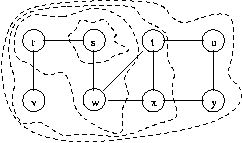
\includegraphics[width=2in]{bfs_example}
\caption{The breadth first search example graph from the Boost Graph Library.  The concentric regions show the order in which breadth first search will visit the vertices.}
\label{fig:bfs}
\end{figure}

We will load the graph from Figure~\ref{fig:bfs} and compute the breadth first search (BFS).

\begin{mcode}
>> load graphs\bfs_example.mat
>> [d dt pred] = bfs(A,2);
>> [ignore order] = sort(dt);
>> labels(order)
ans = 
    's'
    'r'
    'w'
    'v'
    't'
    'x'
    'u'
    'y'
\end{mcode}

The first command loads the graph from the stored representation in Matlab.  As we've seen, we present the graph as a sparse adjacency matrix.  We can look at the full adjacency matrix using the \mycmd{full} command.

\begin{mcode}
>> full(A)
ans =
     0     1     0     0     1     0     0     0     0
     0     0     0     0     1     0     0     0     0
     0     0     0     0     0     1     0     0     0
     0     0     0     0     0     0     0     0     0
     1     0     1     1     0     1     0     0     0
     0     0     0     0     1     0     0     0     0
     0     0     0     0     0     0     0     1     1
     0     0     0     0     0     0     0     0     1
     0     0     0     0     0     0     1     0     0
\end{mcode}

The second command runs the MatlabBGL \mycmd{bfs} command starting from vertex 2.  Looking at the label file, we can see that vertex 2 was really $s$ in the original graph.  The \mycmd{bfs} command returns three vectors: \mycmd{d} is a vector of the distance to each other vertex from $s$; \mycmd{dt} is the discover time of each vertex, the time when the BFS first reached that vertex; and \mycmd{pred} is the predecessor array encoded as a Matlab tree.  In fact, we can view the predecessor array using the \mycmd{treeplot} command.

\begin{mcode}
>> treeplot(pred)
\end{mcode}
\begin{center}
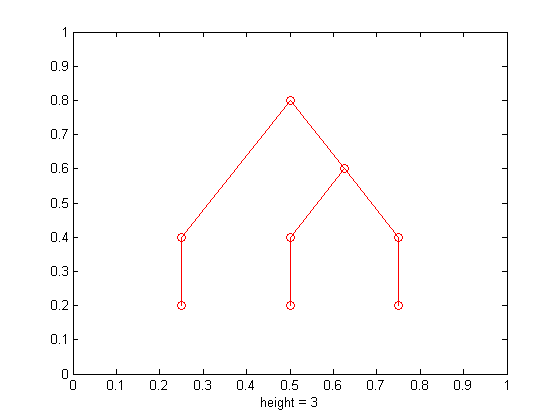
\includegraphics[width=3in]{bfs_treeplot}
\end{center}

The third line of the example sorts the vertices by their discover time and saves the permutation of the indices.  The permutation tells us how to permute the labels array to view the vertex labels in the discover order.  The final line actually prints the labels in their discover order.  Comparing with the original figure, we can see that the vertices were discovered in the correct BFS order.

\subsection{Depth first search}

In this example, we will compute a depth first search (DFS) of the graph in Figure~\ref{fig:dfs}.  This example is implemented in the \mypath{examples/dfs\_example.m} file.

\begin{figure}[ht!]
\centering
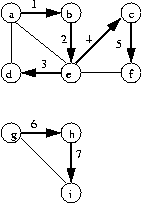
\includegraphics[width=1.25in]{dfs}
\caption{The depth first search example graph from the Boost Graph Library.}
\label{fig:dfs}
\end{figure}

We first load the graph and then call the MatlabBGL \mycmd{dfs} command.  
\begin{mcode}
>> load graphs/dfs_example.mat
>> [d dt ft pred] = dfs(A,1,struct('full',1));
>> [ignore order] = sort(dt);
>> labels(order)
ans = 
    'a'
    'b'
    'e'
    'c'
    'f'
    'd'
    'g'
    'h'
    'i'
\end{mcode}

The \mycmd{dfs} command is similar to the \mycmd{bfs} command.  However, the \mycmd{dfs} routine provides the \mycmd{ft} vector which indicates the finish time for each vertex as well.  The other commands in this script are explained in the first example. 

The graph in Figure~\ref{fig:dfs} is disconnected.  We can use the \mycmd{dfs} command to find all the vertices connected to a source vertex.  

\begin{mcode}
>> load graphs/dfs_example.mat
>> d = dfs(A,1);
>> labels(d < 0)
ans = 
    'g'
    'h'
    'i'
\end{mcode}

This result indicates that nodes $g$, $h$, and $i$ are in a separate component from vertex $a$.  

\subsection{Max-flox min-cut}
The Boost Graph Library provides an implementation of Goldberg's push-relabel maximum flow algorithm.  In this example, we use the \mycmd{max_flow} routine to find the maximum flow of the graph from Figure~\ref{fig:mincut}.  This example is implemented in the \mypath{examples/max\_flow\_example.m} file.  

\begin{figure}[ht!]
\centering
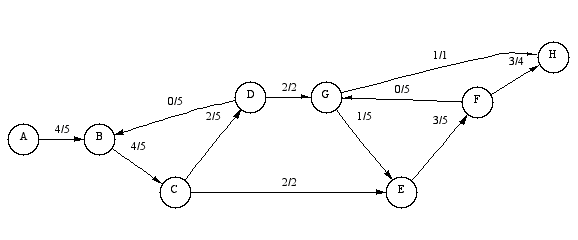
\includegraphics[width=4in]{max-flow}
\caption{The max-flow min-cut example graph from the Boost Graph Library.}
\label{fig:mincut}
\end{figure}

\begin{mcode}
>> load graphs/max_flow_example.mat
>> max_flow(A,1,8)
ans =
     4
>> [flow cut R F] = max_flow(A,1,8);
>> full(R)     
ans =
     0     1     0     0     0     0     0     0
     0     0     1     0     0     0     0     0
     0     0     0     3     0     0     0     0
     0     5     0     0     0     0     0     0
     0     0     0     0     0     2     0     0
     0     0     0     0     0     0     5     1
     0     0     0     0     4     0     0     0
     0     0     0     0     0     0     0     0
\end{mcode}

The script presents two results from the \mycmd{max_flow} routine.  The first call computes the maximum flow from $A$ to $H$.  The second call prints the residual flow graph $R$.  In comparison with Figure~\ref{fig:mincut}, the residual shows the unused capacity on each edge. On the edge from $A$ to $B$, there is only one unit of unused flow, so $R(1,2) = 1$.  

\subsection{New algorithms}
In this section, we will implement a new algorithm using the core set of routines provided by the MatlabBGL library.

\paragraph{Multiway Cut}

The Matlab code for this example is in the file \mypath{examples/multiway\_example.m}.  
Given an undirected graph $G=(V,E)$ with weighted edges $w$.  The multiway cut problem is to find a minimum cost set of edges, $C$, to remove that will disconnect a subset of vertices $S$ from each other.  That is, after we remove the edges $C$ from $G$, there is no path from any vertex $s \in S$ to any other vertex in $S$.  

This problem is NP-complete, but we can find a 2-approximation by solving $|S|$ separate max-flow subproblems.\footnote{Approximation Algorithms.  Vijay V. Vazirani.}  Label the vertices in $S$, $s_1, s_2, \ldots, s_k$, so $k = |S|$.  In each max-flow subproblem, we pick vertex $s_i \in S$ and add a new vertex $t$.  For each $s_j, j\not=i$, we add a directed edge of infinite capacity from $s_j$ to $t$.  We solve the max-flow problem and add the set of edges in the induced min-cut to the set $C$.  

The MatlabBGL implementation of this algorithm follows.

\begin{mcode}
function C = approx_multiway_cut(A,vs)
function C = approx_multiway_cut(A,vs)
% APPROX_MULTIWAY_CUT Solve a 2-approximation to the multi-way cut problem
% 
% C = approx_multiway_cut(A,vs)
%
% Outputs C, the set of edges cut in a 2-approximation to the multiway cut
% problem.  The multiway-cut problem is to find a minimum cost set of edges
% to disconnect all the vertices in vs from each other.
%
% The non-zero values contain the weight of each edge.
%
% The input A must be a symmetric graph.

if (~isequal(A,A'))
    error('approx_multiway_cut:invalidParameter',...
        'the matrix must be symmetric.');
end;

if (min(min(A)) < 0)
    error('approx_multiway_cut:invalidParameter',...
        'the matrix cannot contain negative weights.');
end;

n = size(A,1);

% this should be larger than any conceivable flow...
int_infinity = sum(sum(A))+2*sum(sum(A(vs,:)))+1;

% initial the cut to nothing.
C = sparse(n,n);

% Get A as an edge list...
[i j v] = find(A);

for (kk=1:length(vs))
    v = vs(kk);
    others = setdiff(vs,v);
    
    % Each flow problem add a fake sink as the n+1 vertex
    Aflow = A;
    Aflow(others,n+1) = int_infinity*ones(length(others),1);
    Aflow(n+1,:) = sparse(n+1,1);
    
    % solve the max-flow problem
    [flow ci] = max_flow(Aflow,v,n+1);
    
    % remove the last (fake) entry from the cut.
    ci = ci(1:end-1);
    
    % construct a value over the edges that is 0 except on the cut, we know
    % all values are positive, so just take the absolute value
    vc = abs(v.*(ci(i)-ci(j)))./2;
    
    % add the set of edges to the cut by constructing a sparse matrix with
    % only the cut edges.
    C = C+ sparse(i, j, vc, n,n);
end;
\end{mcode}

We can use this new algorithm to find a set of roads to remove to disconnect a set of nodes.  The following example loads the road network for Minnesota and chooses a set of 125 vertices, calls the \mycmd{approx_multiway_cut} command above, and then draws the cut using the \mycmd{gplot} command.  

\begin{mcode}
load graphs/minnesota.mat

n = size(A,1);
k1 = 75;
k2 = 50;
start1 = 1;
start2 = 800;
vs1 = start1:start1+k1;
vs2 = start2:start2+k2;
vs = [vs1 vs2];
C = approx_multiway_cut(A,vs);

gplot(triu(A),xy,':');
hold on;
gplot(triu(C),xy,'r-');
plot(xy(vs,1),xy(vs,2),'.');
hold off;
set(gca,'XTick',[]);
set(gca,'YTick',[]);
\end{mcode}

When drawing the graphs, we use the \mycmd{triu} command to only select the upper triangular portion of the adjacency matrix.  Otherwise, Matlab will draw both edges, instead of only one edge.  The figure produced by this program follows.

\begin{center}
\includegraphics[width=3in]{multiway_cut-crop}
\end{center}

\section{In-place Modification/Pass by Reference Library}

To facilitate the visitors implemented in the next section, MatlabBGL includes a pass-by-reference library.  This section describes that library and why it is required for MatlabBGL.  In Matlab, the standard variable passing convention is pass-by-value.  That is, each time Matlab calls a function, it copies all of the function arguments so the caller and the callee have separate copies.\footnote{In fact, Matlab optimizes this procedure and only makes a copy if the callee changes the argument.  This technique is often called ``copy-on-write.''}  One serious side effect is that if a function makes a single change to a large matrix, Matlab must \emph{copy} the entire matrix.  Further, if we wish to return the change to the caller, Matlab must \emph{copy} the changed matrix back!  For a large matrix, this can result in serious overhead as in the following example.

For expository purposes, suppose we have a function that simply increments the first entry in a Matlab matrix.
\begin{mcode}
function a=incr_first(a)
% INCR_FIRST Increment the first entry in a matrix.
a(1) = a(1) + 1;
\end{mcode}
Now, we go a little wild and use the code in the following script \mypath{inplace\_example1.m}.
\begin{mcode}
n = 1000000;
ntrials = 1000;

a = ones(n,1);

tic;
for ii=1:ntrials
    a = incr_first(a);
end
fprintf('Standard Matlab: %f seconds\n', toc);
\end{mcode}
The script produces the following output.
\begin{mcode}
>> inplace_example1
Standard Matlab: 12.375000 seconds
\end{mcode}
Twelve seconds?  To simply increment the first entry in an array 1000 times?  This result is slightly inefficient.

The Inplace/pass-by-reference library remedies this inefficiency.  The Inplace library allows us to makes changes to function arguments \emph{in-place}.  That is, the function arguments are \emph{not copied} and the caller and callee share the same variable and memory.  This style of argument passing is often called ``pass-by-reference.''

We designed the Inplace library to be as close to Matlab syntax as possible.  To ``fix'' the example, we need only make a tiny change.
\begin{mcode}
a = ipdouble(ones(n,1));
\end{mcode}
After this change (and changing the output label), the script produces the output.
\begin{mcode} 
>> inplace_example1
Inplace Calls: 0.062000 seconds
\end{mcode}
Much better!

To be slightly more concrete, the Inplace library provides two classes \mycmd{ipdouble} and \mycmd{ipint32} to create pass-by-reference versions of a \mycmd{double} and \mycmd{int32} matrices and vectors.  To summarize, the following commands all work for \mycmd{ipdouble} and \mycmd{ipint32} vectors as expected.

\begin{mcode}
>> ipd = ipdouble(rand(5)); 
>> ipd                           % display works
>> size(ipd)                     % size works
>> ipd(1,:)                      % subscripting works
>> ipd(1,3:end)                  % subscripting with end works
>> ipd(:) = rand(5)              % assignment works
>> ipd(1,3:end) = ones(1,3)      % partial assignment works
>> ipd(:,1) = pi*ones(5,1)       % partial assignment works
\end{mcode}

The following commands do not work quite as you would expect; however there are alternatives available.  
\begin{mcode}
>> ipd = ipdouble(ones(5)) % create a 5x5 ipdouble of ones
>> y = pi*ones(5,5);       % create another vector 
>> ipd2 = ipdouble(ipd);   % deep copy ipd
>> ipd2 = y;               % error!
\end{mcode}
Unfortunately, the Inplace library does not overload the ``='' operator at the moment, so the final statement does not do quite what you expect.  Instead of copying the contents of \mycmd{y} to \mycmd{ipd2}, it simply overwrites the variable \mycmd{ipd2} with the contents of \mycmd{y}.
Instead, you must use the \mycmd{assign} command.
\begin{mcode}
>> assign(ipd2,y);        % correct!
\end{mcode}

Also, you cannot resize Inplace objects, so the following commands do not work.
\begin{mcode}
>> ipd = ipdouble(ones(5)) % create a 5x5 ipdouble of ones
>> ipd(6,6) = 1;           % error!
\end{mcode}
Currently, there is no workaround for this behavior.  Use \mycmd{ipdouble}s like Fortran arrays, which have fixed size.

Finally, there are some syntactic issues when you update an entire \mycmd{ipdouble} or \mycmd{ipint32} vector.
\begin{mcode}
>> ipd = ipdouble(pi*ones(5));  % create a 5x5 ipdouble of pi's
>> ipd = ipd + 1;               % error!
>> ipd = double(ipd) + 1;       % hidden error
>> assign(ipd,ipd(:)+1);        % correct!
\end{mcode}
The first error results because the \mycmd{plus} command is not implemented for the \mycmd{ipdouble} type.  This omission may be fixed in future releases.
The second ``fix'' succeeds but contains a hidden error.  The error is that the type of the result is a Matlab double, not an \mycmd{ipdouble}.  Finally, using the assign command results in the correct behavior.

\section{Visitors}
The visitor feature of the Boost Graph Library is one of the most powerful and subtle features.  By attaching visitors to some of the algorithms, you can \emph{record} or \emph{alter} behavior of the underlying algorithm.  Internally, the Boost Graph Library uses visitors to implement: \mycmd{connected_components}, \mycmd{strong_components}, \mycmd{biconnected_components}, \mycmd{prim_minimum_spanning_tree},  and \mycmd{dijkstra_shortest_paths}.  Using an appropriate visitor and data structure, all these algorithms \emph{could} be implemented natively in Matlab just like the Boost versions.\footnote{Of course, actually implemented them natively in Matlab would negate the performance benefit of using the Boost Graph Library.}

The MatlabBGL library implements visitors using function handles.
\begin{mcode}
>> load graphs/bfs_example.mat
>> ev_func = @(u) fprintf('called examine_vertex(%s)\n', char(labels(u)));
>> bfs_visitor = struct();
>> bfs_visitor.examine_vertex = ev_func;
>> breadth_first_search(A,1,bfs_visitor);
called examine_vertex(r)
called examine_vertex(s)
called examine_vertex(v)
called examine_vertex(w)
called examine_vertex(t)
called examine_vertex(x)
called examine_vertex(u)
called examine_vertex(y)
\end{mcode}

In the following sections, we will describe how MatlabBGL implements visitors with a high level overview and a few examples.  

\subsection{Overview} In the Boost graph library and in MatlabBGL, the following algorithms support visitors:
\begin{itemize}
\item \mycmd{breadth_first_search}
\item \mycmd{depth_first_search}
\item \mycmd{dijkstra_shortest_paths}
\item \mycmd{bellman_ford_shortest_paths}
\item \mycmd{astar_search}.
\end{itemize}
All visitors implemented in Boost are implemented in MatlabBGL.  For the details on the visitors, see the Boost graph library documentation.  Whereas the BGL uses classes and structures to implement visitors, MatlabBGL uses function handles and structures.  

To demonstrate the relationship, we will implemente the \mycmd{bacon_number_recorder} visitor from the Boost graph library examples.\footnote{\url{http://www.boost.org/libs/graph/doc/kevin_bacon.html}}
The algorithm used to determine Bacon numbers is breadth first search.  In the breadth first search algorithm, a tree-edge indicates when the algorithm finds a new shortest path between the start node and another (previously) unknown node.  In terms of Bacon numbers, these events indicate when we find another actor and give us that the Bacon number of the new actor is one greater than the Bacon number of the previous actor.

\begin{mcode}
  template <typename DistanceMap>
  class bacon_number_recorder : public default_bfs_visitor
  {
  public:
    bacon_number_recorder(DistanceMap dist) : d(dist) { }

    template <typename Edge, typename Graph>
    void tree_edge(Edge e, const Graph& g) const
    {
      typename graph_traits<Graph>::vertex_descriptor
	u = source(e, g), v = target(e, g);
	d[v] = d[u] + 1;
    }
  private:
      DistanceMap d;
  };
  // Convenience function
  template <typename DistanceMap>
  bacon_number_recorder<DistanceMap>
  record_bacon_number(DistanceMap d)
  {
    return bacon_number_recorder<DistanceMap>(d);
  }
\end{mcode}

To use the visitor, we need to allocate storage and call breadth first search starting from Kevin Bacon.

\begin{mcode}  
  // allocate storage
  std::vector<int> bacon_number(num_vertices(g));
  
  // call bfs
  Vertex src = actors["Kevin Bacon"];
  bacon_number[src] = 0;

  breadth_first_search(g, src, visitor(record_bacon_number(&bacon_number[0])));
\end{mcode}  

The following code implements the same visitor pattern in MatlabBGL and uses the Inplace library described in the previous section.

\begin{mcode}
function bn = bacon_numbers(A,u)
% BACON_NUMBERS Compute the Bacon numbers for a graph.
%
% bn = bacon_numbers(A,u) computes the Bacon numbers for all nodes in the 
% graph assuming that Kevin Bacon is node u.

% allocate storage for the bacon numbers
% the ipdouble call allocates storage that can be modified in place.
bn_inplace = ipdouble(zeros(num_vertices(A),1));

% implement a nested function that can refer to variables we declare.  In
% this case, we refer to the bn_inplace variable.  
function tree_edge(ei,u,v)
    bn_inplace(v) = bn_inplace(u)+1;
end

% setup the bacon_recorder visitor
bacon_recorder = struct();
bacon_recorder.tree_edge = @tree_edge;

% call breadth_first_search
breadth_first_search(A,u,bacon_recorder);

% convert the inplace storage back to standard Matlab storage to return.
bn = double(bn_inplace);

% the end line is required with nested functions to terminate the file
end
\end{mcode}
The code for the MatlabBGL \mycmd{bacon_number} function is in the \mypath{examples/} subdirectory.  Instead of declaring a class with a member variable \mycmd{d} for the \mycmd{bacon_number_recorder}, the MatlabBGL code uses a \emph{nested function} along with an \mycmd{ipdouble} variable from the Inplace library to accomplish the same behavior.  

\subsection{Specifics}
The Boost graph library has two types of visitor functions \emph{vertex} visitors and \emph{edge} visitors.  A common vertex visitor is the \mycmd{examine_vertex} function.  For the BFSVisitor concept, the Boost graph library defines the following prototype for that visitor.
\begin{mcode}
void visitor::examine_vertex(Vertex u, Graph& g)
\end{mcode}
The corresponding MatlabBGL function takes only one argument, the vertex index.
\begin{mcode}
visitor.examine_vertex = @(u) fprintf('called examine_vertex(%i)!\n', u);
\end{mcode}
In MatlabBGL, the \emph{vertex} visitors follow this same pattern, the only argument is the index of the vertex.

The second type of visitor function, the \emph{edge} visitors have more differences with Boost.  The Boost edge visitor functions provide the Edge datatype directly.  Because MatlabBGL does not define an Edge datatype like the Boost graph library, this call makes no sense.  Instead, the MatlabBGL edge visitor functions provide the \emph{transposed} edge index, the source of the edge, and the target of the edge.  
\begin{mcode}
visitor.examine_edge = @(ei,u,v) ...
    fprintf('called examine_edge(%i,%i,%i)!\n', ei, u, v);
\end{mcode}
First, the edge index is less useful than it may seem initially.  Instead of the edge index into the original graph, the edge index is in the transposed graph that MatlabBGL is using for the computation.  (See section~\ref{sec:impl-details}, you get the transposed edge index unless you tell MatlabBGL not to transpose the graph.))  There is more about this issue in the next paragraph.  The second and third arguments, \mycmd{u} and \mycmd{v} are the source and target of the edge, respectively.  These two variables are quite useful and let you know which vertices the edge touches.  In the most general terms, the edge is a directed edge from vertex $u$ to vertex $v$.  

In fact, there are two issues with the edge index.  First, the edge index comes from the transposed graph.  The second issue is that for an undirected graph, each edge has two indices (one for the forward edge, and one for the reverse edge).  To see a full discussion of both of these issues, see the edge index example in section~\ref{sec:visitors-examples}.


\paragraph{Stopping the Algorithm} At any point, if a visitor function returns a zero value, the algorithm halts.  Often, this behavior may be desirable.  Consider the following example with \mycmd{astar_search}.
\begin{mcode}
load graphs/bgl_cities.mat
goal = 11; % Binghamton
start = 9; % Buffalo
% Use the euclidean distance to the goal as the heuristic
h = @(u) norm(xy(u,:) - xy(goal,:));
% Setup a routine to stop when we find the goal
ev = @(u) (u ~= goal);
[d pred f] = astar_search(A, start, h, ...
    struct('visitor', struct('examine_vertex', ev)));
\end{mcode}
The \mycmd{examine_vertex} function returns 0 when the vertex is a targeted vertex.  In this example, we want to find the shortest path between Binghamton and Buffalo.  Once we find a shortest path to Buffalo, we can halt the algorithm!

In summary, 
\begin{itemize}
\item MatlabBGL visitor function have the same names as the Boost graph library visitor functions;
\item vertex visitor functions provide only the index of the vertex, e.g. \mycmd{examine_vertex(u)};
\item edge visitor functions provide the \emph{transposed} \mycmd{edge_index} and the two endpoints of the edge, \mycmd{u} and \mycmd{v}, e.g. \mycmd{examine_edge(ei,u,v)};
\item the Inplace library and nested functions are useful tools to implement visitors; and
\item visitor function can halt an algorithm by returning 0.
\end{itemize}

For additional discussion of some of the implementation details, see section~\ref{subsec:mbgl-bfs}~and~\ref{subsec:visitor-edges}.

\subsection{Examples}
\label{sec:visitors-examples}
In this section, we give three examples to demonstrate how to use the visitor library.  First, we have an example that outputs messages from all events to show how an algorithm works.  Second, we have an example that demonstrates how to \emph{correctly} use edge-indices in the visitors.  Finally, the breadth-first-search example reimplements the \mycmd{bfs} function using MatlabBGL visitors instead of Boost graph library visitors.

\subsubsection*{Recording algorithm behavior}

 In this example, we will write a simple visitor that outputs an
 algorithm's behavior.  The algorithm we will examine is \mycmd{dijkstra_sp}.  To
 examine the runtime behavior we will use a visitor which outputs a string
 every time a function is called.


%% Setup
 To begin, we load a graph.

\begin{mcode}
>> load graphs/clr-25-2.mat
\end{mcode}

%%
 Next, let's check the documentation to see which functions to implement 
 for the visitor

\begin{mcode}
>> help dijkstra_sp
...
  visitor is a struct with the following optional fields
     vis.initialize_vertex(u)
     vis.discover_vertex(u)
     vis.examine_vertex(u)
     vis.examine_edge(ei,u,v)
     vis.edge_relaxed(ei,u,v)
     vis.edge_not_relaxed(ei,u,v)
     vis.finish_vertex(u)
...     
\end{mcode}

%%
 The help states that \mycmd{dijkstra_sp} allows visitors functions for
 \mycmd{initialize_vertex}, \mycmd{discover_vertex}, \mycmd{examine_vertex}, \mycmd{examine_edge},
 \mycmd{edge_relaxed}, \mycmd{edge_not_relaxed}, and \mycmd{finish_vertex}.

 Rather than implementing 7 functions ourselves, we define two helper
 functions.  These helper functions return functions themselves.  There is
 one helper that returns a vertex visitor function and one helper than
 returns an edge visitor function.

\begin{mcode}
>> vertex_vis_print_func = @(str) @(u) ...
      fprintf('%s called on %s\n', str, char(labels{u}));
>> edge_vis_print_func = @(str) @(ei,u,v) ...
      fprintf('%s called on (%s,%s)\n', str, char(labels{u}), char(labels{v}));
\end{mcode}

%% 
% These anonymous functions return functions themselves.

\begin{mcode}
>> ev_func = vertex_vis_print_func('examine_vertex');
>> ev_func(1)
examine_vertex called on s
\end{mcode}

%% 
 I hope you see how these functions are useful in saving quite a bit of
 typing.

%% Calling dijkstra_sp
 We are almost done.  Now, we just have to setup the visitor structure to
 pass to the \mycmd{dijkstra_sp} call.

\begin{mcode}
>> vis = struct();
>> vis.initialize_vertex = vertex_vis_print_func('initialize_vertex');
>> vis.discover_vertex = vertex_vis_print_func('discover_vertex');
>> vis.examine_vertex = vertex_vis_print_func('examine_vertex');
>> vis.finish_vertex = vertex_vis_print_func('finish_vertex');
>> vis.examine_edge = edge_vis_print_func('examine_edge');
>> vis.edge_relaxed = edge_vis_print_func('edge_relaxed');
>> vis.edge_not_relaxed = edge_vis_print_func('edge_not_relaxed');
\end{mcode}

%%
 With the visitor setup, there is hardly any work left.  

\begin{mcode}
>> dijkstra_sp(A,1,struct('visitor', vis));
discover_vertex called on s
examine_vertex called on s
examine_edge called on (s,u)
edge_relaxed called on (s,u)
discover_vertex called on u
examine_edge called on (s,x)
edge_relaxed called on (s,x)
discover_vertex called on x
finish_vertex called on s
examine_vertex called on u
examine_edge called on (u,x)
edge_not_relaxed called on (u,x)
examine_edge called on (u,v)
edge_relaxed called on (u,v)
discover_vertex called on v
finish_vertex called on u
examine_vertex called on x
examine_edge called on (x,u)
examine_edge called on (x,v)
edge_not_relaxed called on (x,v)
examine_edge called on (x,y)
edge_relaxed called on (x,y)
discover_vertex called on y
finish_vertex called on x
examine_vertex called on v
examine_edge called on (v,y)
edge_not_relaxed called on (v,y)
finish_vertex called on v
examine_vertex called on y
examine_edge called on (y,s)
examine_edge called on (y,v)
finish_vertex called on y
\end{mcode}

% Understanding the output
 To understand the output, we find it helpful to have a copy of
 Introduction to Algorithms by Cormen, Leiserson, and Rivest.  The source
 for the graph is Figure 25-2 in that book and the authors use the graph
 to illustrate how Dijkstra's algorithm runs.  In particular, Figure 25-5
 shows a sample run of Dijkstra's algorithm.

 Perhaps the first thing to notice is that the initialize vertex visitor
 is never called.  This results from an error in the MatlabBGL and Boost
 documentation.  Once it is resolved, we will update the MatlabBGL
 documentation to match the Boost graph library.

 The results: \mycmd{discover_vertex} is called before \mycmd{examine_vertex}, 
 except for the source node $u$. For the edges, \mycmd{examine_edge} is always called before either \mycmd{edge_relaxed}
 or \mycmd{edge_not_relaxed}.  The edges that are relaxed are the shaded edges in
 Figure 25-5.

 Finally, \mycmd{finish_vertex} is called on a vertex after all of its edges have
 been examined and possibly relaxed.  	
 
 This example is implemented in the file \mypath{examples/record\_alg.m}.
 

\subsubsection*{Reimplementing \mycmd{bfs}}
\label{subsec:mbgl-bfs}

 For this example, we will implement the \mycmd{bfs} command using the \mycmd{breadth_first_search} routine along with a set of visitors.  The visitors will record
 \begin{enumerate}
 \item the distance in edges from a source vertex to a destination vertex,
 \item the predecessor of each vertex in the search tree, and
 \item the discovery time of each vertex.
 \end{enumerate}
 At the end, we benchmark this search against the MatlabBGL \mycmd{bfs} function to estimate the performance impact of the Matlab visitors.
 
 	The begin the algorithm, we have to initialize a series of vectors to store the data.
 	\begin{mcode}
ip_d = -ones(num_vertices(A),1);
ip_dt = -ones(num_vertices(A),1);
ip_pred = zeros(1,num_vertices(A));
ip_time = ipdouble(1);
 	\end{mcode}
 	The \mycmd{bfs} function requires that \mycmd{ip_d} and \mycmd{ip_dt} are $-1$ if a vertex is not reachable from the starting vertex, so we initialize those arrays with $-1$.  The \mycmd{ip_pred} array is 0 if a vertex is not in the BFS tree.  The \mycmd{ip_time} variable is used to keep a running index of how many steps the algorithm takes.
 	
 	With our arrays constructed, we can build visitor functions to update each of the arrays.  We won't go through the details of the following visitors, but they implement the \mycmd{time_stamper}, \mycmd{distance_recorder}, and \mycmd{predecessor_recorder} visitors from the BGL.	 These functions are nested functions, so they refer to variables in the outer variable scope.
 	\begin{mcode}
function time_discover_vertex(u)
    ip_dt(u) = ip_time(1);
    ip_time(1) = ip_time(1) + 1;
end

function distance_tree_edge(ei,u,v)
    ip_d(v) = ip_d(u)+1;
end

function pred_tree_edge(ei,u,v)
    ip_pred(v) = u;
end 	
\end{mcode}
  With the visitor function, we simply construct the visitors by creating a set of structures and using the \mycmd{combine_visitors} function.
\begin{mcode}
vis_distance = struct('tree_edge', @distance_tree_edge);
vis_time = struct('discover_vertex', @time_discover_vertex);
vis_pred = struct('tree_edge', @pred_tree_edge);

vis = combine_visitors(vis_distance, vis_time, vis_pred);
\end{mcode}
The only remaining task is to call the \mycmd{breadth_first_search} algorithm.  Prior to making the call, we must finish some brief initialization to properly denote the source vertex.
\begin{mcode}
ip_d(u) = 0;
ip_dt(u) = ip_time(1);

breadth_first_search(A,u,vis);
\end{mcode}  
After the call to \mycmd{breadth_first_search}, the desired data remains in the \mycmd{ip_d}, \mycmd{ip_dt}, and \mycmd{ip_pred} variables.  To finish, we convert these to real \mycmd{double} times from the \mycmd{ipdouble} types used in the algorithms.

 The \mycmd{bfs_in_mbgl} function is provided in the \mypath{examples/} directory.  We can use this implementation to benchmark the performance difference between the Matlab based visitor implementation and the native visitor implementation.  
	\begin{mcode}
% from the examples subdirectory	
>> load ../graphs/minnesota.mat
>> tic;
>> [d dt pred] = bfs(A,1);
>> toc;
>> tic;
>> [d dt pred] = bfs_in_mbgl(A,1);
>> toc;
Elapsed time is 0.000000 seconds.
Elapsed time is 2.469000 seconds.
\end{mcode}
Unfortunately, there is significant overhead in calling the MatlabBGL visitors, and the MatlabBGL implementation is much slower on even a small graph (2642 vertices).  Nevertheless, the interactive computation environment in Matlab offers significant speed advantages and reduced development time.

\paragraph{Becoming more efficient} The previous example was needlessly inefficient.  Here, we explain how to implement the previous example in a faster and more efficient manner.  First, the \mycmd{combine_visitors} function is a nice general function, but there is overhead involved in each call to the visitor.  Also, there is an alternative to using the Inplace library for the visitors which yields a slight performance increase.

Briefly, we define the arrays without the Inplace library.
\begin{mcode}
ip_d = -ones(num_vertices(A),1);
ip_dt = -ones(num_vertices(A),1);
ip_pred = zeros(1,num_vertices(A));

ip_time = 1;
\end{mcode}
Then, we define a single pair of nested functions which perform all the visitor tasks.
\begin{mcode}
function discover_vertex(u)
    ip_dt(u) = ip_time(1);
    ip_time(1) = ip_time(1) + 1;
end

function tree_edge(ei,u,v)
    ip_d(v) = ip_d(u)+1;
    ip_pred(v) = u;
end
\end{mcode}
Finally, we construct the visitor structure, setup the initial values for each variable, and call \mycmd{breadth_first_search}.
\begin{mcode}
vis = struct('discover_vertex', @discover_vertex, 'tree_edge', @tree_edge);

ip_d(u) = 0;
ip_dt(u) = ip_time(1);

breadth_first_search(A,u,vis);
\end{mcode}
The code for the efficient version is in the \mycmd{bfs_in_mbgl_efficient} function is provided in the \mypath{examples/} directory.  Using this version, we recompute the timings.
\begin{mcode}
% from the examples subdirectory	
>> load ../graphs/minnesota.mat
>> tic;
>> [d dt pred] = bfs(A,1);
>> toc;
>> tic;
>> [d dt pred] = bfs_in_mbgl_efficient(A,1);
>> toc;
Elapsed time is 0.000000 seconds.
Elapsed time is 0.469000 seconds.
\end{mcode}
These small changes have made a considerable change in the runtime of the function.  While the native code is still considerably faster, the new code is an improvement.

To reiterate, the code for this example is implemented in the \mycmd{bfs_in_mbgl} and \mycmd{bfs_in_mbgl_efficient} functions in the \mypath{examples/} directory.

\subsubsection*{Edge index example}
\label{subsec:visitor-edges}

 This example is, perhaps, the most intricate.  Here, we will delve into how to use the edge index provided in the edge visitor functions.  
 
 To begin, let's determine the problem.  Suppose we have a graph with a numeric value associated with each edge.  One example would be a weighted graph, however, this example is intended to be fairly general.  Effectively, we will describe how to work with edge property maps and MatlabBGL.
 As always, we need a graph to use.
 \begin{mcode}
>> load graphs/bfs_example.mat 
\end{mcode}

 Now we assign a random value to each edge in the graph.  
\begin{mcode} 
>> [i,j,val] = find(A);
>> edge_rand = rand(num_edges(A),1);
\end{mcode}
 Presently, we have an implicit association between edges and values.  That is, each directed edge in \mycmd{A} has a separate value.  In the next statement, we make the mapping concrete and explicitly indicate which value we want for each edge.\footnote{This step is not required or recommended.  We perform this step to be completely concrete about the intended mapping.  In your own code, you should always maintain the mapping implicitly for the highest performance.}
\begin{mcode}
>> Av = sparse(i, j, edge_rand, size(A,1), size(A,2));
\end{mcode}

The first case we demonstrate is the ``obvious'' usage, but contains an error.  We define an edge visitor to write out some data on every edge the algorithm examines.
\begin{mcode}
>> ee = @(ei,u,v) fprintf(...
    'examine_edge   %2i,   %1i,   %1i,   %4f,   %4f\n', ...
    ei, u, v, edge_rand(trans_ei_to_ei(ei)), Av(u,v));
\end{mcode}    
Also, let's write a quick heading so that we can read and understand the the output before we call the \mycmd{breadth_first_search} algorithm.
\begin{mcode}
>> fprintf('               ei,   u,   v,     er(ei),true er(ei)\n');
>> breadth_first_search(A,1,struct('examine_edge',ee));
               ei,   u,   v,     er(ei),     A(u,v)
examine_edge    1,   1,   2,   0.950129,   0.606843
examine_edge    2,   1,   5,   0.231139,   0.444703
examine_edge    3,   2,   1,   0.606843,   0.950129
examine_edge    4,   2,   6,   0.485982,   0.615432
examine_edge   10,   5,   1,   0.444703,   0.231139
...
\end{mcode}
Quickly, we can see that using the edge index itself does not give us the correct mapping between edges and edge-values. Recall that \mycmd{A(u,v)} was the intended value, but all the edge values are stored with an implicit order in \mycmd{edge_rand}.  
\mynote{The edge index cannot be trivially used to index edge values.}

In order to make the edge index return the correct value, we must define an \emph{edge index map}.  In Matlab, this means we need to create a vector with an entry for each edge in the graph such that the entry indexed by the transposed edge index returns the actual edge index.  Effectively, we want to undo the transposition that occurs when we use the MatlabBGL library.\footnote{If you use the \mycmd{notrans} option, then this section may or may not apply to you.}
We can efficiently construct the map using the following two commands.
\begin{mcode}
>> [i,j,val] = find(A);
>> Aind = sparse(i,j,1:num_edges(A),size(A,1), size(A,2));
>> [i,j,trans_ei_to_ei] = find(Aind');
\end{mcode}  
These lines create a new sparse matrix with the same sparsity pattern as \mycmd{A}, but where each value is replaced by its edge index.  To create the edge index map, we simply read out the transposed matrix into a value array.  

With the edge index map in hand, we can correctly code the previous example.
\begin{mcode}
>> ee = @(ei,u,v) fprintf('examine_edge   %2i,   %1i,   %1i,   %4f,   %4f\n', ...
       ei, u, v, edge_rand(trans_ei_to_ei(ei)), Av(u,v));
>> fprintf('               ei,   u,   v,     er(ei),true er(ei)\n');
>> breadth_first_search(A,1,struct('examine_edge',ee));
               ei,   u,   v,     er(ei),true er(ei)
examine_edge    1,   1,   2,   0.202647,   0.202647
examine_edge    2,   1,   5,   0.502813,   0.502813
examine_edge    3,   2,   1,   0.846221,   0.846221
examine_edge    4,   2,   6,   0.709471,   0.709471
examine_edge   10,   5,   1,   0.525152,   0.525152
...
\end{mcode}
The code now correctly indexes the \mycmd{edge_rand} array and gets the correct value for each edge.

The first two examples assumed that each edge $(u,v)$ and $(v,u)$ have distinct values.  Instead, suppose we have a single value for both $(u,v)$ and $(v,u)$ and only store half of them.  We need to build a \mycmd{trans_ei_to_ei} map that correct handles this case as well.  The only change is that we only deal with the upper triangular part of the matrix instead of the full matrix.  The following code computes an appropriate \mycmd{trans_ei_to_ei} to index a new 
\mycmd{edge_rand} vector that is defined for each undirected edge.

\begin{mcode}
>> [i,j,val] = find(triu(A,1));
>> edge_rand = rand(num_edges(A)/2,1);
>> % build a tranposed edge index to edge index map
>> Aind = sparse([i; j],[j; i],[1:num_edges(A)/2 1:num_edges(A)/2], size(A,1), size(A,2));
>> [i,j,trans_ei_to_ei] = find(Aind');
>> ee = @(ei,u,v) fprintf('examine_edge   %2i,   %1i,   %1i,   %4f,   %4f\n', ...
>>     ei, u, v, edge_rand(trans_ei_to_ei(ei)), edge_rand(Aind(u,v)));
>> fprintf('               ei,   u,   v,     er(ei),true er(ei)\n');
>> breadth_first_search(A,1,struct('examine_edge',ee));
               ei,   u,   v,     er(ei),true er(ei)
examine_edge    1,   1,   2,   0.150873,   0.150873
examine_edge    2,   1,   5,   0.378373,   0.378373
examine_edge    3,   2,   1,   0.150873,   0.150873
examine_edge    4,   2,   6,   0.860012,   0.860012
examine_edge   10,   5,   1,   0.378373,   0.378373
...
\end{mcode}
In this output, notice that $(1,2)$ and $(2,1)$ both map to the same set of values.  







 This example is implemented in the file \mypath{examples/edge\_index\_example.m}.

\section{Features not implemented}

This section contains a list of features that I think should be in MatlabBGL and are currently missing.  If you agree, please send me an email.

\begin{itemize}
\item max-flow intermediate data: Currently, the max-flow algorithm generates a large amount of intermediate data that could be cached between calls if the underlying graph does not change.  
\item support for more algorithms from the Boost Graph Library: I chose not to implement more algorithms from Boost until there is demand or time allows.  The matrix ordering commands are redundant in Matlab because they are already built in.
\item edge labeled graph type: The support for graphs with edge labels is limited.  Although the Matlab sparse matrix type easily supports subgraphs, for a graph with edge labels, computing a subgraph is more difficult.  
\item better graph drawing tools: the \mycmd{gplotwl} function in the Matlab File Exchange plots both weights and labels 
\end{itemize}



\section{Reference}

\subsection{Sample Graphs}
This section lists the set of sample graphs provided with MatlabBGL.  The table should be read as \mycmd{clr-26-1.mat} is a directed, weighted graph without labels or node coordinates, the graph came from CLR Figure 26-1.  The source CLR is   The source KT is Kleinberg and Tardos, Algorithm Design, 2006.  
\begin{center}
\begin{tabularx}{\linewidth}{c|cc|cc|X}
\textbf{Name} & \textbf{Dir.} & \textbf{Weighted} & \textbf{Labels} & \textbf{Coords.} & \textbf{Source}\\
\hline
clr-24-1 & & $\times$ & $\times$ & $\times$ & CLR\footnote{Corman, Leiserson, and Rivest. Introduction
 to Algorithms, 2nd Edition.} Fig. 24.1\\
clr-25-2 & $\times$ & $\times$ & $\times$ & & CLR Fig. 25.2\\
clr-26-1 & $\times$ & $\times$ & & & CLR Fig. 26.1\\
clr-27-1 &  $\times$ & $\times$ & & & CLR Fig. 27.1\\
kt-3-2 &  &  & & & KT\footnote{ Kleinberg and Tardos. Algorithm Design} Fig. 3.2\\
kt-3-7 & $\times$ &  & & & KT Fig. 3.7\\
kt-6-23 & $\times$ & $\times$ & $\times$ & & KT Fig. 6.23\\
kt-7-2 & $\times$ & $\times$ & $\times$& & KT Fig. 7.2\\
tarjan-biconn & & & & $\times$ & Tarjan\footnote{Tarjan.  Depth-first search and linear graph algorithms, 1972.} Fig. 2\\
padgett-florentine & & & $\times$ & $\times$ &  Website\footnote{\url{http://mrvar.fdv.uni-lj.si/sola/info4/uvod/part4.pdf}}\\
minnesota & & & $\times$ & $\times$ & Highway Data\footnote{National Highway Planning Network, 2003.}\\
tapir & & & & $\times$ & meshpart\footnote{Gilbert and Teng, meshpart toolkit.} \\
cs-stanford & $\times$ & & $\times$ & & Partial webbase 2001 crawl\footnote{Accessed via \url{http://law.dsi.unimi.it/index.php?option=com_include&Itemid=65}.}
\end{tabularx}
\end{center}

\subsection{Functions}

\hrule
\subsection*{Searches}
\vspace{1cm}
\hrule
\subsubsection*{bfs}
\begin{mcode}
  BFS Compute the breadth first search order.
 
  [d dt pred] = bfs(A,u) returns the distance to each vertex (d) and the  
  discover time (dt) in a breadth first search starting from vertex u.
     d(i) = dt(i) = -1 if vertex i is not reachable from vertex u.
  pred is the predecessor array.  pred(i) = 0 if vertex (i)  
  is in a component not reachable from u and i != u.
 
  This method works on directed graphs.
  The runtime is O(V+E).
 
  ... = bfs(A,u,options) sets optional parameters (see 
  set_matlab_bgl_options) for the standard options.
    There are no additional options for this function.
 
  Note: this function does not depend upon the non-zero values of A, but
  only uses the non-zero structure of A.
 
  Example:
     load graphs/bfs_example.mat
     d = bfs(A,1)
 
  See also DFS
\end{mcode}
\newpage
\subsubsection*{dfs}
\begin{mcode}
  DFS Compute the depth first search times.
 
  [d dt ft pred] = dfs(A,u) returns the distance (d), the discover (dt) and
  finish time (ft) for each vertex in the graph in a depth first search 
  starting from vertex u.
    d = dt(i) = ft(i) = -1 if vertex i is not reachable from u
  pred is the predecessor array.  pred(i) = 0 if vertex (i)  
  is in a component not reachable from u and i != u.
  
  ... = dfs(A,u,options) sets optional parameters (see 
  set_matlab_bgl_options) for the standard options.
    options.full: compute the full dfs instead of the dfs of
       the current component (see Note 1) [{0} | 1]
 
  Note 1: When computing the full dfs, the vertex u is ignored, vertex 1 is
  always used as the starting vertex.  
 
  Note: this function does not depend upon the non-zero values of A, but
  only uses the non-zero structure of A.
 
  Example:
     load graphs/dfs_example.mat
     d = dfs(A,1)
 
  See also BFS
\end{mcode}
\newpage
\subsubsection*{breadth\_first\_search}
\begin{mcode}
  BREADTH_FIRST_SEARCH Fully wrap the Boost breadth_first_search call
  including the bfs_visitor.
 
  breadth_first_search(A,u,vis) performs a breadth first traversal 
  of A starting from vertex u.  For each event defined by the bfs_visitor 
  structure below, the visitor is called with the either the name of the 
  vertex (u), or the edge index and it's source and target (ei,u,v).  
 
  See http://www.boost.org/libs/graph/doc/BFSVisitor.html for a description
  of the events.
  
  bfs_visitor is a struct with the following optional fields
     vis.initialize_vertex(u)
     vis.discover_vertex(u)
     vis.examine_vertex(u)
     vis.examine_edge(ei,u,v)
     vis.tree_edge(ei,u,v)
     vis.non_tree_edge(ei,u,v)
     vis.gray_target(ei,u,v)
     vis.black_target(ei,u,v)
     vis.finish_vertex(u)
  Each bfs_visitor parameter should be a function pointer, which returns 0
  if the bfs should stop.  (If the function does not return anything, the
  bfs continues.)
 
  This method works on directed graphs.
  The runtime is O(V+E), excluding the complexity of the visitor
  operations.
 
  Realistically, this function must be used with the
  pass-by-reference/in-place modification library.  
 
  ... = breadth_first_search(A,u,vis,options) sets optional parameters (see 
  set_matlab_bgl_options) for the standard options.
    There are no additional options for this function.
 
  Note: this function does not depend upon the non-zero values of A, but
  only uses the non-zero structure of A.
 
  Example:
    This example finds the distance to a single point and stops the search.
    function dist_uv(A,u,v,options)
      vstar = v;
      dmap = ipdouble(zeros(size(A,1),1));
      function stop=on_tree_edge(ei,u,v)
        dmap[v] = dmap[u]+1;
        return (v ~= vstar);
      end;
      breadth_first_search(A,u,struct('tree_edge',@on_tree_edge),options);
    end;
 
  See also BFS
\end{mcode}
\newpage
\subsubsection*{depth\_first\_search}
\begin{mcode}
  DEPTH_FIRST_SEARCH Fully wrap the Boost depth_first_search call
  including the dfs_visitor.
 
  depth_first_search(A,u,dfs_visitor) performs a depth first traversal 
  of A starting from vertex u.  For each event defined by the dfs_visitor 
  structure below, the visitor is called with the either the name of the 
  vertex (u), or the edge index and it's source and target (ei,u,v).  
 
  See http://www.boost.org/libs/graph/doc/DFSVisitor.html for a description
  of the events.
  
  dfs_visitor is a struct with the following optional fields
     vis.initialize_vertex(u)
     vis.start_vertex(u)
     vis.discover_vertex(u)
     vis.examine_edge(ei,u,v)
     vis.tree_edge(ei,u,v)
     vis.back_edge(ei,u,v)
     vis.forward_or_cross_edge(ei,u,v)
     vis.finish_vertex(u)
  Each dfs_visitor parameter should be a function pointer, which returns 0
  if the dfs should stop.  (If the function does not return anything, the
  dfs continues.)
 
  This method works on directed graphs.
  The runtime is O(V+E), excluding the complexity of the visitor
  operations.
 
  Realistically, this function must be used with the
  pass-by-reference/in-place modification library.  
 
  ... = depth_first_search(A,u,vis,options) sets optional parameters (see 
  set_matlab_bgl_options) for the standard options.
    options.full: compute the full dfs instead of the dfs of
       the current component (see Note 1) [{0} | 1]
 
  Note 1: When computing the full dfs, the vertex u is ignored, vertex 1 is
  always used as the starting vertex.  
 
  Note: this function does not depend upon the non-zero values of A, but
  only uses the non-zero structure of A.
 
  Example:
    This example finds the distance to a single point and stops the search.
    function dist_uv(A,u,v,options)
      vstar = v;
      dmap = ipdouble(zeros(size(A,1),1));
      function stop=on_tree_edge(ei,u,v)
        dmap[v] = dmap[u]+1;
        return (v ~= vstar);
      end;
      breadth_first_search(A,u,struct('tree_edge',@on_tree_edge),options);
    end;
 
  See also DFS
\end{mcode}
\newpage
\hrule
\subsection*{Components}
\vspace{1cm}
\hrule
\subsubsection*{components}
\begin{mcode}
  Simulink components.
 
  slmdldiscui   - Launch Simulink Model Discretizer UI
  sldiscmdl     - Discretize Simulink model block by block 


components is both a directory and a function.

  COMPONENTS Compute the connected components of a graph.
 
  [ci sizes] = components(A) returns the component index vector (ci) and
  the size of each of the connected components (sizes).  The number of
  connected components is max(components(A)).  The algorithm used computes
  the strongly connected components of A, which are the connected
  components of A if A is undirected (i.e. symmetric).  
 
  This method works on directed graphs.
  The runtime is O(V+E), the algorithm is just depth first search.
 
  ... = components(A,options) sets optional parameters (see 
  set_matlab_bgl_options) for the standard options.
    There are no additional options for this function.
 
  Note: this function does not depend upon the non-zero values of A, but
  only uses the non-zero structure of A.
 
  Example: 
     load graphs/dfs_example.mat
     components(A)
 
  See also DMPERM, BICONNECTED_COMPONENTS
\end{mcode}
\newpage
\subsubsection*{biconnected\_components}
\begin{mcode}
  BICONNECTED_COMPONENTS Compute the biconnected components and
  articulation points for a symmetric graph A.
 
  [a C] = biconnected_components(A) returns a list of articulation points 
  a and the component graph C where each non-zero indicates the connected
  component of the edge.  That is, C is a matrix with the same non-zero
  structure as A, but with the values replaced with the index of the
  biconnected component of that edge.  The vector a is a list of
  articulation points in the graph.  Articulation points are vertices that
  belong to more than one biconnected component.  Removing an articulation
  point disconnects the graph.
 
  If C is not requested, it is not built.
 
  This method works on undirected graphs.
  The runtime is O(V+E), the algorithm is just depth first search.
 
  ... = biconnected_components(A,optionsu) sets optional parameters (see 
  set_matlab_bgl_options) for the standard options.
    There are no additional options for this function.
 
  Note: the input to this function must be symmetric, so this function
  ignores the 'notrans' default option and never transposes the input.
 
  Note: this function does not depend upon the non-zero values of A, but
  only uses the non-zero structure of A.
 
  Example:
     load graphs/tarjan-biconn.mat
     biconnected_components(A)
 
  See also COMPONENTS
\end{mcode}
\newpage
\hrule
\subsection*{Shortest Paths}
\vspace{1cm}
\hrule
\subsubsection*{shortest\_paths}
\begin{mcode}
  SHORTEST_PATHS Compute the weighted single source shortest path problem.
 
  [d pred] = shortest_paths(A,u) returns the distance (d) and the predecessor
  (pred) for each of the vertices along the shortest path from u to every
  other vertex in the graph.  
  
  ... = shortest_paths(A,u,options) sets optional parameters (see 
  set_matlab_bgl_options) for the standard options.
    options.algname: the algorithm to use 
        [{'auto'} | 'dijkstra' | 'bellman_ford' | 'dag']
    options.inf: the value to use for unreachable vertices 
        [double > 0 | {Inf}]
    options.visitor: a structure with visitor callbacks.  This option only
        applies to dijkstra or bellman_ford algorithms.  See dijkstra_sp or
        bellman_ford_sp for details on the visitors.
    options.edge_weight: a double array over the vertices with an edge
        weight for each node
 
  Note: 'auto' cannot be used with 'nocheck' = 1.  The 'auto' algorithm
  checks if the graph has negative edges and uses bellman_ford in that
  case, otherwise, it uses 'dijkstra'.  In the future, it may check if the
  graph is a dag and use 'dag'.  
 
  Example:
     load graphs/clr-25-2.mat
     shortest_paths(A,1)
     shortest_paths(A,1,struct('algname','bellman_ford'))
 
  See also DIJKSTRA_SP, BELLMAN_FORD_SP, DAG_SP
\end{mcode}
\newpage
\subsubsection*{all\_shortest\_paths}
\begin{mcode}
  all_shortest_paths Compute the weighted all pairs shortest path problem.
 
  D = all_shortest_paths(A) returns the distance matrix D for all vertices
  where D(i,j) indicates the shortest path distance between vertex i and
  vertex j.  
  
  ... = all_shortest_paths(A,u,options) sets optional parameters (see 
  set_matlab_bgl_options) for the standard options.
    options.algname:: the algorithm to use 
        [{'auto'} | 'johnson' | 'floyd_warshall']
    options.inf: the value to use for unreachable vertices 
        [double > 0 | {Inf}]
 
  Note: 'auto' cannot be used with 'nocheck' = 1.  The 'auto' algorithms
  checks the number of edges in A and if the graph is more than 10% dense,
  it uses the Floyd-Warshall algorithm instead of Johnson's algorithm.
 
  Example:
     load graphs/clr-26-1.mat
     all_shortest_paths(A)
     all_shortest_paths(A,struct('algname','johnson'))
 
  See also JOHNSON_ALL_SP, FLOYD_WARSHALL_ALL_SP.
\end{mcode}
\newpage
\subsubsection*{dijkstra\_sp}
\begin{mcode}
  DIJKSTRA_SP Compute the weighted single source shortest path problem.
 
  Dijkstra's algorithm for the single source shortest path problem only
  works on graphs without negative edge weights.
 
  This method works on weighted directed graphs without negative edge
  weights.
  The runtime is O(V log (V)).
 
  See the shortest_paths function for calling information.  This function 
  just calls shortest_paths(...,struct('algname','dijkstra'));
 
  The options structure can contain a visitor for the Dijkstra algorithm.  
 
  See http://www.boost.org/libs/graph/doc/DijkstraVisitor.html for a 
  description of the events.
  
  visitor is a struct with the following optional fields
     vis.initialize_vertex(u)
     vis.discover_vertex(u)
     vis.examine_vertex(u)
     vis.examine_edge(ei,u,v)
     vis.edge_relaxed(ei,u,v)
     vis.edge_not_relaxed(ei,u,v)
     vis.finish_vertex(u)
  Each visitor parameter should be a function pointer, which returns 0
  if the shortest path search should stop.  (If the function does not 
  return anything, the algorithm continues.)
 
  Example:
     load graphs/clr-25-2.mat
     dijkstra_sp(A,1)
 
  See also SHORTEST_PATHS, BELLMAN_FORD_SP.
\end{mcode}
\newpage
\subsubsection*{bellman\_ford\_sp}
\begin{mcode}
  BELLMAN_FORD_SP Compute the weighted single source shortest path problem.
 
  The Bellman-Ford algorithm for the single source shortest path problem
  works on graphs with negative edge weights.  
 
  See the shortest_paths function for calling information.  This function 
  just calls shortest_paths(...,struct('algname','bellman_ford'));
 
  This method works on weighted directed graphs with negative edge weights.
  The runtime is O(VE).
 
  The options structure can contain a visitor for the Bellman-Ford 
  algorithm.  
 
  See http://www.boost.org/libs/graph/doc/BellmanFordVisitor.html for a 
  description of the events.
  
  visitor is a struct with the following optional fields
     vis.initialize_vertex(u)
     vis.examine_edge(ei,u,v)
     vis.edge_relaxed(ei,u,v)
     vis.edge_not_relaxed(ei,u,v)
     vis.edge_minimized(ei,u,v)
     vis.edge_not_minimized(ei,u,v)
  Each visitor parameter should be a function pointer, which returns 0
  if the shortest path search should stop.  (If the function does not 
  return anything, the algorithm continues.)
 
  Example:
     load graphs/kt-6-23.mat
     d = bellman_ford_sp(A,1);
 
  See also SHORTEST_PATHS, DIJKSTRA_SP.
\end{mcode}
\newpage
\subsubsection*{dag\_sp}
\begin{mcode}
  DAG_SP Compute the weighted single source shortest path problem.
 
  The DAG shortest path algorithm for the single source shortest path
  problem only works on directed acyclic-graphs (DAGs).  
 
  If the graph is not a DAG, the results are undefined.  In the future, the
  function may throw an error if the graph is not a DAG.
 
  See the shortest_paths function for calling information.  This function 
  just calls shortest_paths(...,struct('algname','dag'));
 
  This algorithm works on weighted directed acyclic graphs.
  The runtime is O(V+E)
 
  ... = clustering_coefficients(A,options) sets optional parameters (see 
  set_matlab_bgl_options) for the standard options.
     There are no additional options for this function.
 
  Example:
     load graphs/kt-3-7.mat
     dag_sp(A,1)
 
  See also SHORTEST_PATHS
\end{mcode}
\newpage
\subsubsection*{johnson\_all\_sp}
\begin{mcode}
  JOHNSON_ALL_SP Compute the weighted all-pairs shortest path problem.
 
  Johnson's algorithm for the all-pairs shortest path problem 
  works only on graphs without negative edge weights.  This method should
  be used over the Floyd-Warshall algorithm for sparse graphs.  
 
  This method works on weighted directed graphs.
  The runtime is O(VE log(V)).
 
  See the shortest_paths function for calling information.  This function 
  just calls all_shortest_paths(...,struct('algname','johnson'));
 
  Example:
     load graphs/clr-26-1.mat
     johnson_all_sp(A)
 
  See also ALL_SHORTEST_PATHS, FLOYD_WARSHALL_ALL_SP.
\end{mcode}
\newpage
\subsubsection*{floyd\_warshall\_all\_sp}
\begin{mcode}
  FLOYD_WARSHALL_ALL_SP Compute the weighted all-pairs shortest path problem.
 
  The Floyd-Warshall algorithm for the all-pairs shortest path problem 
  works only on graphs without negative edge weights.  This method should
  be used over the Johnson algorithm for dense graphs.  
 
  This method works on weighted directed graphs.
  The runtime is O(V^3).
 
  See the shortest_paths function for calling information.  This function 
  just calls all_shortest_paths(...,struct('algname','floyd_warshall'));
 
  Example:
     load graphs/clr-26-1.mat
     floyd_warshall_all_sp(A)
 
  See also ALL_SHORTEST_PATHS, JOHNSON_ALL_SP.
\end{mcode}
\newpage
\subsubsection*{astar\_search}
\begin{mcode}
  ASTAR_SEARCH Perform a heuristically guided (A*) search on the graph.
 
  [d pred rank]=astar_search(A,s,h,optionsu) returns the distance map,
  search tree and f-value of each node in an astar_search. 
  The search begins at vertex s.  The heuristic h guides the search, 
  h(v) should be small close to a goal and large far from a goal.  The
  heuristic h can either be a vector with an entry for each vertex in the
  graph or a function which maps vertices to values.
 
  This method works on non-negatively weighted directed graphs.
  The runtime is O((E+V)log(V)).
 
  ... = astar_search(A,u,options) sets optional parameters (see 
  set_matlab_bgl_options) for the standard options.
    options.visitor: a visitor to use with the A* search (see Note)
    options.inf: the value to use for unreachable vertices 
        [double > 0 | {Inf}]
    
  Note: You can specify a visitor for this algorithm.  The visitor has the
  following optional functions.
     vis.initialize_vertex(u)
     vis.discover_vertex(u)
     vis.examine_vertex(u)
     vis.examine_edge(ei,u,v)
     vis.edge_relaxed(ei,u,v)
     vis.edge_not_relaxed(ei,u,v)
     vis.black_target(ei,u,v)
     vis.finish_vertex(u)
  Each visitor parameter should be a function pointer, which returns 0
  if the search should stop.  (If the function does not return anything, 
  the algorithm continues.)
 
  Example:
    load graphs/bgl_cities.mat
    goal = 11; % Binghamton
    start = 9; % Buffalo
    % Use the euclidean distance to the goal as the heuristic
    h = @(u) norm(xy(u,:) - xy(goal,:));
    % Setup a routine to stop when we find the goal
    ev = @(u) (u ~= goal);
    [d pred f] = astar_search(A, start, h, ...
        struct('visitor', struct('examine_vertex', ev)));
\end{mcode}
\newpage
\hrule
\subsection*{Minimum Spanning Trees}
\vspace{1cm}
\hrule
\subsubsection*{mst}
\begin{mcode}
  MST Compute a minimum spanning tree for an undirected graph A.
 
  There are two ways to call MST.
  T = mst(A)
  [i j v] = mst(A) 
  The first call returns the minimum spanning tree T of A.  
  The second call returns the set of edges in the minimum spanning tree.  
  The calls are related by 
     T = sparse(i,j,v,size(A,1), size(A,1)); 
     T = T + T';
  The optional algname parameter chooses which algorithm to use to compute
  the minium spanning tree.  Note that the set of edges returned is not
  symmetric and the final graph must be explicitly symmetrized.
 
  This method works on undirected graphs graphs.
 
  ... = mst(A,optionsu) sets optional parameters (see 
  set_matlab_bgl_options) for the standard options.
    options.algname: the minimum spanning tree algorithm
      ['prim' | {'kruskal'}]
 
  Note: the input to this function must be symmetric, so this function
  ignores the 'notrans' default option and never transposes the input.
 
  Example:
     load graphs/clr-24-1.mat
     mst(A)
 
  See also PRIM_MST, KRUSKAL_MST
\end{mcode}
\newpage
\subsubsection*{kruskal\_mst}
\begin{mcode}
  KRUSKAL_MST Compute a minimum spanning with Kruskal's algorithm.
 
  The Kruskal MST algorithm computes a minimum spanning tree for a graph.
 
  This method works on weighted symmetric graphs.
  The runtime is O(E log (E)).
 
  See the mst function for calling information.  This function just calls
  mst(...,struct('algname','kruskal'));
 
  Example:
     load graphs/clr-24-1.mat
     kruskal_mst(A)
 
  See also MST, PRIM_MST.
\end{mcode}
\newpage
\subsubsection*{prim\_mst}
\begin{mcode}
  PRIM_MST Compute a minimum spanning with Kruskal's algorithm.
 
  Prim's MST algorithm computes a minimum spanning tree for a graph.
 
  This method works on weighted symmetric graphs without negative edge
  weights.
  The runtime is O(E log (V)).
 
  See MST for calling information.  This function just calls
  mst(...,struct('algname','prim'));
 
  Example:
     load graphs/clr-24-1.mat
     prim_mst(A)
 
  See also MST, KRUSKAL_MST.
\end{mcode}
\newpage
\hrule
\subsection*{Statistics}
\vspace{1cm}
\hrule
\subsubsection*{num\_edges}
\begin{mcode}
  NUM_EDGES The number of edges in a graph.
 
  n = num_edges(A) returns the number of edges in graph A.  
 
  For symmetric/undirected graphs, the number of edges returned is twice 
  the number of undirected edges.
 
  Example:
     load graphs/dfs_example.mat
     n = num_edges(A)
 
  See also NUM_VERTICES
\end{mcode}
\newpage
\subsubsection*{num\_vertices}
\begin{mcode}
  NUM_VERTICES The number of vertices in a graph.
 
  n = num_vertices(A) returns the number of vertices in graph A.  
 
  Example:
     A = sparse(ones(5));
     n = num_vertices(A);
 
  See also NUM_EDGES
\end{mcode}
\newpage
\subsubsection*{clustering\_coefficients}
\begin{mcode}
  CLUSTERING_COEFFICIENTS Compute the clustering coefficients for vertices.
 
  ccfs = clustering_coefficients(A) returns the clustering coefficients for
  all vertices in A.  The clustering coefficient is the ratio of the number
  of edges between a vertex's neighbors to the total possible number of 
  edges between the vertex's neighbors. 
 
  This method works on directed or undirected graphs.
  The runtime is O(nd^2) where d is the maximum vertex degree.
 
  ... = clustering_coefficients(A,options) sets optional parameters (see 
  set_matlab_bgl_options) for the standard options.
    There are no additional options for this function.
 
  Note: this function does not depend upon the non-zero values of A, but
  only uses the non-zero structure of A.
 
  Example:
     load graphs\clique-10.mat
     clustering_coefficients(A)
\end{mcode}
\newpage
\subsubsection*{betweenness\_centrality}
\begin{mcode}
  BETWEENNESS_CENTRALITY Compute the betweenness centrality for vertices.
 
  bc = betweenness_centrality(A) returns the betweenness centrality for
  all vertices in A.  
 
  [bc,E] = betweenness_centrality(A) returns the betweenness centrality for
  all vertices in A along with a sparse matrix with the centrality for each
  edge.  
 
  This method works on weighted or weighted directed graphs.
  For unweighted graphs (options.unweighted=1), the runtime is O(VE).
  For weighted graphs, the runtime is O(VE + V(V+E)log(V)).
 
  ... = betweenness_centrality(A,options) sets optional parameters (see 
  set_matlab_bgl_options) for the standard options.
    options.unweighted: use the slightly more efficient unweighted
      algorithm in the case where all edge-weights are equal [{0} | 1]  
    options.ec_list: do not form the sparse matrix with edge [{0} | 1]
 
  Note: the edge centrality can also be returned as an edge list using the
  options.ec_list options.  This option can eliminate some ambiguity in the
  output matrix E when the edge centrality of an edge is 0 and Matlab drops
  the edge from the sparse matrix.  
 
  Note: if the edge centrality matrix E is not requested, then it is not
  computed and not returned.  This yields a slight savings in computation
  time.  
 
  Example:
     load graphs/padgett-florentine.mat
     betweenness_centrality(A)
\end{mcode}
\newpage
\hrule
\subsection*{Flow}
\vspace{1cm}
\hrule
\subsubsection*{max\_flow}
\begin{mcode}
  MAX_FLOW Compute the max flow on A from u to v.
 
  flowval=max_flow(A,u,v) computes the maximum flow on the network defined by
  the adjacency structure A, with source u and sink v.
 
  [flowval cut R F] = max_flow(A,u,v) returns the maximum flow in the 
  network A with source u and sink v as well as additional information.  
  For each vertex on the source side of the mincut, mincut(i) = 1, 
  for each vertex on the sink side, mincut(i) = -1.  
  R is the residual graph.  R(i,j) is the amount of unused capacity 
  on edge (i,j).  F is the flow graph, F(i,j) is the amount of used 
  capacity on edge (i,j).  F, A, and R satisfy the relationship A = F + R.
 
  The algorithm used is the push-relabel algorithm.
 
  ... = max_flow(A,optionsu) sets optional parameters (see 
  set_matlab_bgl_options) for the standard options.
    There are no additional options for this function.
 
  Note: the values on A are interpreted as integers, please round them
  yourself to get the best interpretation.  The code uses the floor of 
  the values in A.
 
  Example:
     load graphs\max_flow_example.mat
     max_flow(A,1,8)
\end{mcode}
\newpage
\hrule
\subsection*{Graphs}
\vspace{1cm}
\hrule
\subsubsection*{erdos\_reyni}
\begin{mcode}
  ERDOS_REYNI Generates a random Erdos-Reyni (Gnp) graph
 
  A=erdos_reyni(n,p) generates a random Gnp graph with n vertices and where
  the probability of each edge is p.  The resulting graph is symmetric.
 
  This function is different from the Boost Graph library version, it was
  reimplemented natively in Matlab.
 
  Example:
    A = erdos_reyni(100,0.05);
\end{mcode}
\newpage
\subsubsection*{cycle\_graph}
\begin{mcode}
  CYCLE_GRAPH Generate the cycle graph of order n
 
  The cycle graph is a simple cycle with n vertices.
 
  [A xy] = cycle_graph(n) generates a cycle graph with n vertices and
  returns the adjacency matrix in A.  The matrix xy stores two-dimensional 
  coordinates for each vertex.
 
  Example:
    [A xy] = cycle_graph(10);
    gplot(A,xy);
 
  See also WHEEL_GRAPH, STAR_GRAPH
\end{mcode}
\newpage
\subsubsection*{star\_graph}
\begin{mcode}
  STAR_GRAPH Generate the star graph of order n
 
  The star graph is a simple star with n vertices.  Vertex n is the center
  vertex.
 
  [A xy] = star_graph(n) generates a star graph with n vertices and
  returns the adjacency matrix in A.  The matrix xy stores two-dimensional 
  coordinates for each vertex.
 
  Example:
    [A xy] = star_graph(10);
    gplot(A,xy);
 
  See also WHEEL_GRAPH, CYCLE_GRAPH
\end{mcode}
\newpage
\subsubsection*{wheel\_graph}
\begin{mcode}
  WHEEL_GRAPH Construct a wheel graph of order n
 
  The wheel graph is a cycle graph of order n-1 along with an additional
  vertex that connects all the remaining vertices.  (Run the example and it
  will be extremely clear if you are still confused.)
 
  [A xy] = wheel_graph(n) returns the adjacency matrix for the wheel graph
  of order n.  The matrix xy stores two-dimensional coordinates for each 
  vertex.
 
  Example:
    [A xy] = wheel_graph(10);
    gplot(A,xy);
 
  See also CYCLE_GRAPH, STAR_GRAPH
\end{mcode}
\newpage
\hrule
\subsection*{Visitors}
\vspace{1cm}
\hrule
\subsubsection*{combine\_visitors}
\begin{mcode}
  COMBINE_VISITORS Generate a new visitor by combining existing visitors
 
  cv = combine_visitors(v1, v2, ...) generates a new algorithm visitor that
  works by calling the functions in v1 followed by the functions in v2, and
  so on.  
 
  The value returned by the combined visitor function is the bitwise & of
  all the individual return values.  So, if any visitor requests the
  algorithm to halt, then the algorithm will halt.
 
  Note: using a combined visitor is somewhat slower than writing a custom
  combined visitor yourself.
 
  Example:
     vis1 = struct();
     vis1.examine_vertex = @(u) fprintf('vis1: examine_vertex(%i)\n', u);
     vis2 = struct();
     vis2.examine_vertex = @(u) fprintf('vis2: examine_vertex(%i)\n', u);
     combined_vis = combine_visitors(vis1, vis2);
     load graphs/bfs_example.mat
     breadth_first_search(A,1,combined_vis);
\end{mcode}
\newpage
\hrule
\subsection*{Options}
\vspace{1cm}
\hrule
\subsubsection*{set\_matlab\_bgl\_default}
\begin{mcode}
  SET_MATLAB_BGL_DEFAULT Sets a default option for the Matlab BGL interface
 
  old_default = set_matlab_bgl_default(options)
  options.istrans: the input matrices are already transposed [{0} | 1]
  options.nocheck: skip the input checking [{0} | 1]
  options.full2sparse: convert full matrices to sparse [{0} | 1]
 
  to get the current set of default options, call
  options = set_matlab_bgl_default()
 
  These options can make the Matlab BGL interface more efficient by
  eliminating the copying operations that occur between Matlab's structures
  and the BGL structures.  However, they are more difficult to use and are
  disabled by default.
 
  Generally, they are best used when you want to perform a large series of
  computations.
 
  e.g.
  % tranpose the matrix initially...
  At = A'
  old_options = set_matlab_bgl_default(struct('istrans',1));
  % perform a bunch of graph work with At...
  d1 = dfs(At,1); d2 = dfs(At,2); ...
  % restore the old options 
  set_matlab_bgl_default(old_options);
\end{mcode}

\end{document}